\documentclass{article}
\usepackage{tikz}
\usepackage{subfig}
\usepackage[margin=1.0in]{geometry}
\pagestyle{empty}
\begin{document}


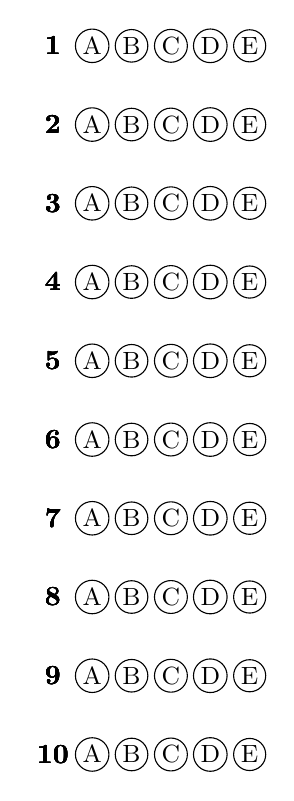
\begin{tikzpicture}[font=\small]
    \foreach \line in {1,2,...,10} {
        \begin{scope}[yshift=-\line cm]
            \foreach \letter/\position in {A/1, B/2, C/3, D/4, E/5} { 
                \node at (0,0) {\normalsize\textbf{\line}};
                \node[draw,circle,inner sep=1pt] at ({\position * 0.5},0) {\letter};
            }
        \end{scope}
    }
\end{tikzpicture}\hfill
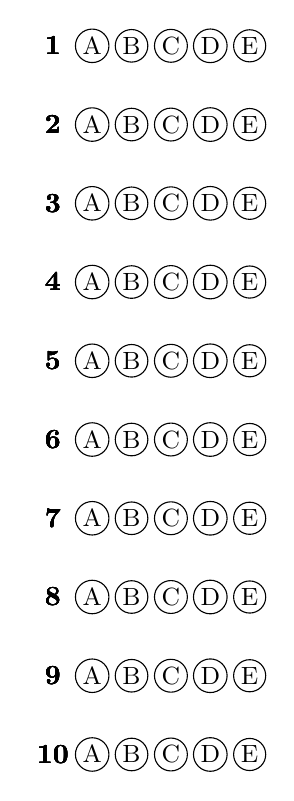
\begin{tikzpicture}[font=\small]
    \foreach \line in {1,2,...,10} {
        \begin{scope}[yshift=-\line cm]
            \foreach \letter/\position in {A/1, B/2, C/3, D/4, E/5} { 
                \node at (0,0) {\normalsize\textbf{\line}};
                \node[draw,circle,inner sep=1pt] at ({\position * 0.5},0) {\letter};
            }
        \end{scope}
    }
\end{tikzpicture}
\vfill
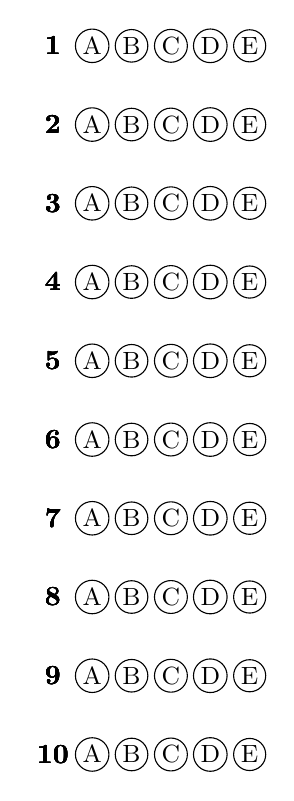
\begin{tikzpicture}[font=\small]
    \foreach \line in {1,2,...,10} {
        \begin{scope}[yshift=-\line cm]
            \foreach \letter/\position in {A/1, B/2, C/3, D/4, E/5} { 
                \node at (0,0) {\normalsize\textbf{\line}};
                \node[draw,circle,inner sep=1pt] at ({\position * 0.5},0) {\letter};
            }
        \end{scope}
    }
\end{tikzpicture}\hfill
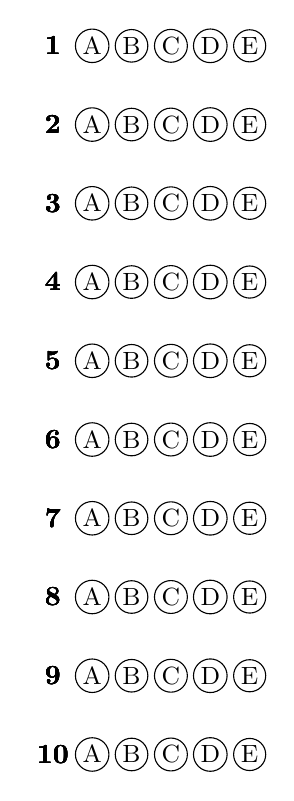
\begin{tikzpicture}[font=\small]
    \foreach \line in {1,2,...,10} {
        \begin{scope}[yshift=-\line cm]
            \foreach \letter/\position in {A/1, B/2, C/3, D/4, E/5} { 
                \node at (0,0) {\normalsize\textbf{\line}};
                \node[draw,circle,inner sep=1pt] at ({\position * 0.5},0) {\letter};
            }
        \end{scope}
    }
\end{tikzpicture}
\end{document}